%%%%%%%%%%%%%%%%%%%%%%%%%%%%%%%%%%%%%%%%%
% Make sure to set your name, legi number and url to the right git branch.
\newcommand{\hmwkAuthorName}{Alberto Montes} % Your name
\newcommand{\hmwkAuthorLegi}{16-932-451} % Your name
\newcommand{\hmwkGitBranch}{\texttt{16-932-451/1\_locally\_linear\_embedding}} % Your name
%
%%%%%%%%%%%%%%%%%%%%%%%%%%%%%%%%%%%%%%%%%

%----------------------------------------------------------------------------------------
%	PACKAGES AND OTHER DOCUMENT CONFIGURATIONS
%	Skip this
%----------------------------------------------------------------------------------------

\documentclass{article}

\usepackage{fancyhdr} % Required for custom headers
\usepackage{lastpage} % Required to determine the last page for the footer
\usepackage{extramarks} % Required for headers and footers
\usepackage{graphicx} % Required to insert images
\usepackage{subcaption}
\usepackage{float}
\usepackage{lipsum} % Used for inserting dummy 'Lorem ipsum' text into the template

\usepackage{amsmath}
\usepackage{amssymb}
\newcommand{\vect}[1]{\mathbf{#1}}
% \newcommand{\Real}{\mathbb{R}}


% Margins
\topmargin=-0.45in
\evensidemargin=0in
\oddsidemargin=0in
\textwidth=6.5in
\textheight=9.0in
\headsep=0.25in

\linespread{1.1} % Line spacing

% Set up the header and footer
\pagestyle{fancy}
\lhead{\hmwkAuthorName} % Top left header
\chead{\hmwkClass\ \hmwkTitle} % Top center header
\rhead{\firstxmark} % Top right header
\lfoot{\lastxmark} % Bottom left footer
\cfoot{} % Bottom center footer
\rfoot{Page\ \thepage\ of\ \pageref{LastPage}} % Bottom right footer
\renewcommand\headrulewidth{0.4pt} % Size of the header rule
\renewcommand\footrulewidth{0.4pt} % Size of the footer rule

\setlength\parindent{0pt} % Removes all indentation from paragraphs

%----------------------------------------------------------------------------------------
%	DOCUMENT STRUCTURE COMMANDS
%	Skip this
%----------------------------------------------------------------------------------------

% Header and footer for when a page split occurs within a problem environment
\newcommand{\enterProblemHeader}[1]{
\nobreak\extramarks{#1}{#1 continued on next page\ldots}\nobreak
\nobreak\extramarks{#1 (continued)}{#1 continued on next page\ldots}\nobreak
}

% Header and footer for when a page split occurs between problem environments
\newcommand{\exitProblemHeader}[1]{
\nobreak\extramarks{#1 (continued)}{#1 continued on next page\ldots}\nobreak
\nobreak\extramarks{#1}{}\nobreak
}

\setcounter{secnumdepth}{0} % Removes default section numbers
\newcounter{homeworkProblemCounter} % Creates a counter to keep track of the number of problems

\newcommand{\homeworkProblemName}{}
\newenvironment{homeworkProblem}[1][Problem \arabic{homeworkProblemCounter}]{ % Makes a new environment called homeworkProblem which takes 1 argument (custom name) but the default is "Problem #"
\stepcounter{homeworkProblemCounter} % Increase counter for number of problems
\renewcommand{\homeworkProblemName}{#1} % Assign \homeworkProblemName the name of the problem
\section{\homeworkProblemName} % Make a section in the document with the custom problem count
\enterProblemHeader{\homeworkProblemName} % Header and footer within the environment
}{
\exitProblemHeader{\homeworkProblemName} % Header and footer after the environment
}

\newcommand{\problemAnswer}[1]{ % Defines the problem answer command with the content as the only argument
\noindent\framebox[\columnwidth][c]{\begin{minipage}{0.98\columnwidth}#1\end{minipage}} % Makes the box around the problem answer and puts the content inside
}

\newcommand{\homeworkSectionName}{}
\newenvironment{homeworkSection}[1]{ % New environment for sections within homework problems, takes 1 argument - the name of the section
\renewcommand{\homeworkSectionName}{#1} % Assign \homeworkSectionName to the name of the section from the environment argument
\subsection{\homeworkSectionName} % Make a subsection with the custom name of the subsection
\enterProblemHeader{\homeworkProblemName\ [\homeworkSectionName]} % Header and footer within the environment
}{
\enterProblemHeader{\homeworkProblemName} % Header and footer after the environment
}

%----------------------------------------------------------------------------------------
%	NAME AND CLASS SECTION
%	Skip this
%----------------------------------------------------------------------------------------

\newcommand{\hmwkTitle}{Locally Linear Embedding} % Assignment title
\newcommand{\hmwkDueDate}{Monday,\ March\ 6th,\ 2017} % Due date
\newcommand{\hmwkClass}{SLT coding exercise\ \#1} % Course/class
\newcommand{\hmwkClassTime}{Mo 16:15} % Class/lecture time
\newcommand{\hmwkClassInstructor}{} % Teacher/lecturer

%----------------------------------------------------------------------------------------
%	TITLE PAGE
%	Skip this
%----------------------------------------------------------------------------------------

\title{
\vspace{2in}
\textmd{\small{\hmwkClass}}\\
\textmd{\textbf{\hmwkTitle}}\\
\small{https://gitlab.vis.ethz.ch/vwegmayr/slt-coding-exercises}\\
\normalsize\vspace{0.1in}\small{Due\ on\ \hmwkDueDate}
%\vspace{0.1in}\large{\textit{\hmwkClassInstructor\ \hmwkClassTime}}
\vspace{3in}
}

\author{
\hmwkAuthorName\\
\hmwkAuthorLegi
}

\date{March 1, 2017} % Insert date here if you want it to appear below your name

\begin{document}

\maketitle

%----------------------------------------------------------------------------------------
%	TABLE OF CONTENTS
%	Skip this
%----------------------------------------------------------------------------------------

%\setcounter{tocdepth}{1} % Uncomment this line if you don't want subsections listed in the ToC

\newpage
\tableofcontents
\newpage

%----------------------------------------------------------------------------------------
%	SECTIONS
%	Now you are in the right hood
%----------------------------------------------------------------------------------------

\begin{homeworkProblem}[The Model]
The model section is intended to allow you to recapitulate the essential ingredients used in \hmwkTitle. Write down the \textit{necessary} equations to specify \hmwkTitle\ and and shortly explain the variables that are involved. This section should only introduce the equations, their solution should be outlined in the implementation section.\newline
Hard limit: One page
\vspace{10pt}

\problemAnswer{ % Answer

Considering a data set of N points D-dimensional $\mathbf{x}_i \in \mathbb{R}^D$. The goal of Locally Linear Embedding is to embed this points into a lower dimensional space $d \ll D$, so to represent each point $\mathbf{x}_i$ with a point $\mathbf{y}_i \in \mathbb{R}^d$. Define a reconstruction error:

\begin{equation}
  E (\mathbf{W}) = \sum_i \| \mathbf{x}_i - \sum_j w_{i j} \mathbf{x}_j \|^2
\end{equation}

Being $j$ the index of the $K$ nearest neighbors of $\mathbf{x}_i$ being $K$ a parameter to tune. As the error want to be invariant to uniform translations, $\mathbf{W}$ has the following restriction: $\sum_j w_{ij} = 1$. $\mathbf{W}$ is computed with the following equation:

\begin{equation}
  w_{ij} = \frac{\sum_k C^{(i)-1}_{jk}}{\sum_{jk} C^{(i)-1}_{lk}} \text{ and } C^{(i)-1}_{lk} = (\mathbf{x}_i - \mathbf{x}_j)^T(\mathbf{x}_i - \mathbf{x}_k)
\end{equation}

Then fixing $\mathbf{W}$ and minimizing the embedding error:

\begin{equation}
  E(\mathbf{y}_1 \ldots \mathbf{y}_N) = \sum_i \| \mathbf{y}_i - \sum_j w_{i j} \mathbf{y}_j \|^2 = \sum_k \mathbf{u}_k^T \mathbf{M} \mathbf{u}_k
\end{equation}

with $\mathbf{u}_k=(y_{ik}, \ldots, y_{Nk})$ for $k=1, \ldots, d$ and $\mathbf{M} = (\mathbf{I} - \mathbf{W})^T (\mathbf{I} - \mathbf{W})$.

The solution of this system correspond to the eigenvectors corresponding to the lowest eigenvalues discarding the first one with eigenvalue $0$.

}
\end{homeworkProblem}
\clearpage

%----------------------------------------------------------------------------------------
\begin{homeworkProblem}[The Questions]
This is the core section of your report, which contains the tasks for this exercise and your respective solutions. Make sure you present your results in an illustrative way by making use of graphics, plots, tables, etc. so that a reader can understand the results with a single glance. Check that your graphics have enough resolution or are vector graphics. Consider the use of GIFs when appropriate.\newline
Hard limit: Two pages

\begin{homeworkSection}{(a) Get the data}
For this exercise we will work with the MNIST data set. In order to learn more about it and download it, go to http://yann.lecun.com/exdb/mnist/.
\end{homeworkSection}

\begin{homeworkSection}{(b) Locally linear embedding}
Implement the LLE algorithm and apply it to the MNIST data set. Provide descriptive visualizations for 2D \& 3D embedding spaces. Is it possible to see clusters?
\end{homeworkSection}

\begin{homeworkSection}{(c) Cluster structure}
Investigate the cluster structure of the data. Can you observe block structures in the $M$ matrix (use matrix plots)? Also plot the singular values of $M$. Do you notice something?
Can you think of ways to determine the optimal embedding dimension?
\end{homeworkSection}

\begin{homeworkSection}{(d) Nearest Neighbors}
Investigate the influence of the choice of how many nearest neighbors you take into account. Additionally, try different metrics to find the nearest neighbors (we are dealing with images!).
\end{homeworkSection}

\begin{homeworkSection}{(e) Linear manifold interpolation}
Assume you pick some point in the embedding space. How can you map it back to the original (high dimensional) space? Investigate how well this works for points within and outside the manifold (does it depend on the dimensionality of the embedding space?) Try things like linearly interpolating between two embedding vectors and plot the sequence of images along that line. What happens if you do that in the original space?
\end{homeworkSection}

\vspace{10pt}
\problemAnswer{ % Answer

The implementation of the algorithm is at \texttt{locally\_linear\_embedding.py} file which computes the embedding for the given data. Lets compute the 2D and 3D embeddings for 1000 samples of the MNIST test dataset. The algorithm computes with 8 nearest neighbor and a euclidean distance

\begin{figure}[H]
\begin{subfigure}{.5\textwidth}
  \centering
  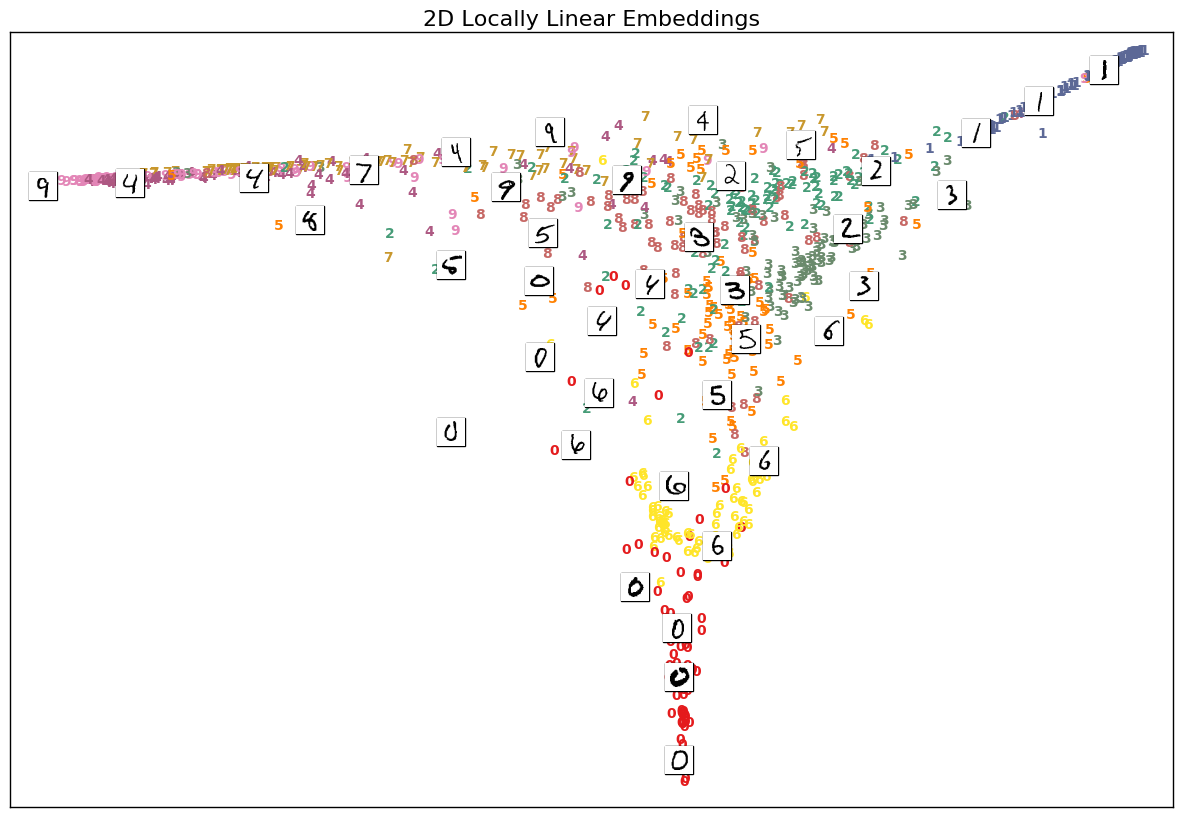
\includegraphics[width=1\linewidth]{images/2d_embeddings}
\end{subfigure}%
\begin{subfigure}{.5\textwidth}
  \centering
  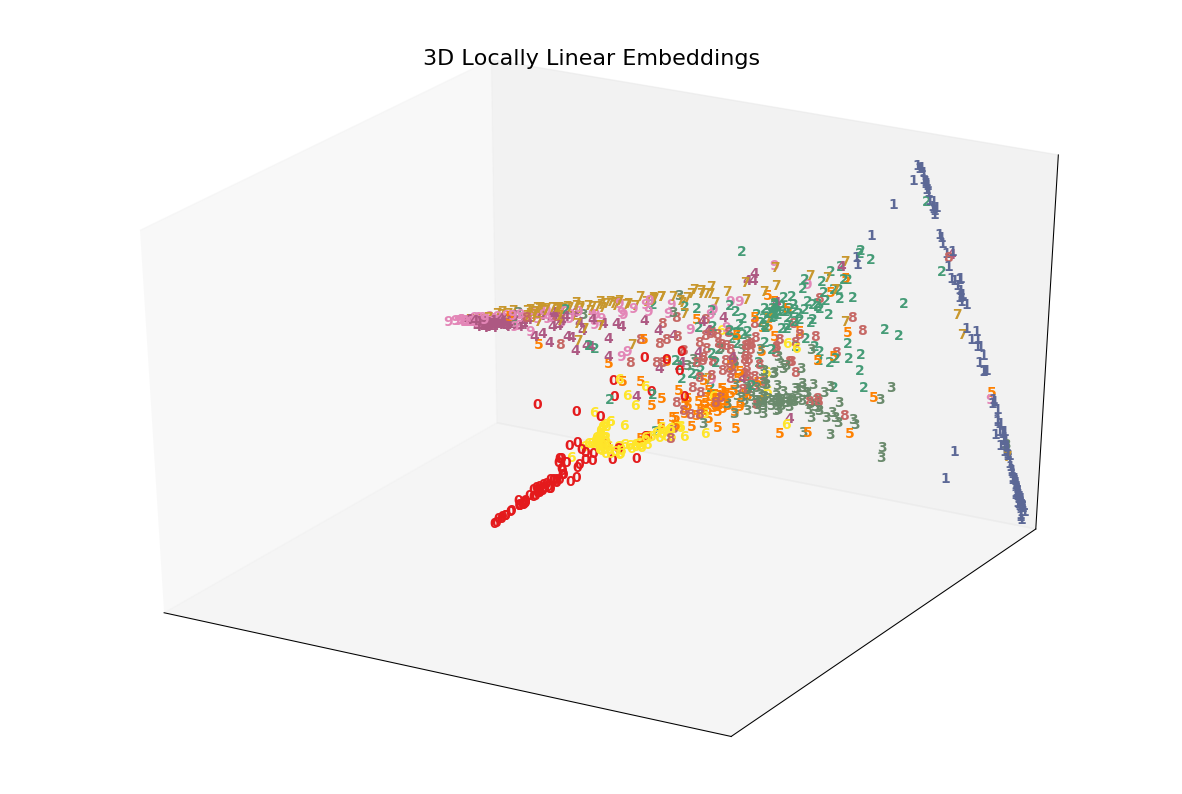
\includegraphics[width=1\linewidth]{images/3d_embeddings}
\end{subfigure}
\caption{2D and 3D Locally Linear Embedding with 8 nearest neighbors}
\label{fig:embeddings}
\end{figure}

On Figure~\ref{fig:embeddings} where the resulting embeddings are shown, it can be easily seen some clusters corresponding to digits, and also how samples with the same digit tent to be close to each other. Also is observed how the digits \texttt{9}, \texttt{0} and \texttt{1} are at the extremes of the manifold as are the most different from the rest. Also can be observed a bunch of other digits close to each other as their shape are very similar.

To see more in deep perspective how clusters are made, in Figure~\ref{fig:matrix_cluster} there is represented the values of the matrix with the columns and rows ordered by the digit of the its correspondent sample.
It can be observed how a lot of correlation between samples of the same digit, and also some cross correlations between digits such as between 4 and 9 or 3 and 5 for example. This results are consistent with the clusters observed at the embeddings.

\begin{figure}[H]
  \begin{subfigure}{.5\textwidth}
    \centering
    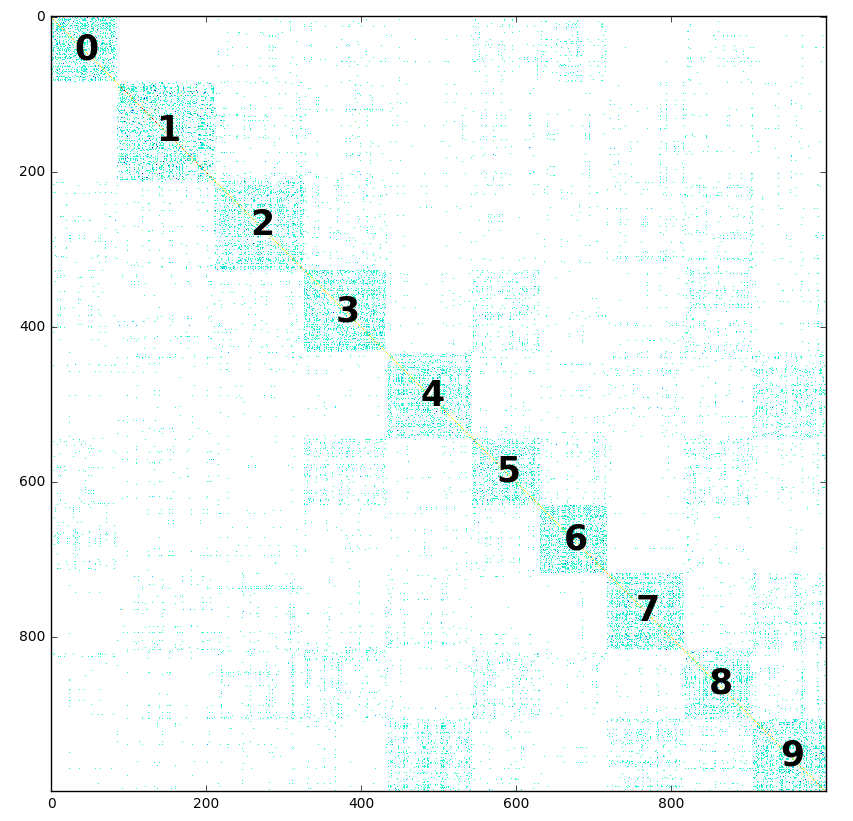
\includegraphics[width=.7\linewidth]{images/matrix_clusters}
    \caption{Matrix plot of $M$.}
    \label{fig:matrix_cluster}
  \end{subfigure}%
  \begin{subfigure}{.5\textwidth}
    \centering
    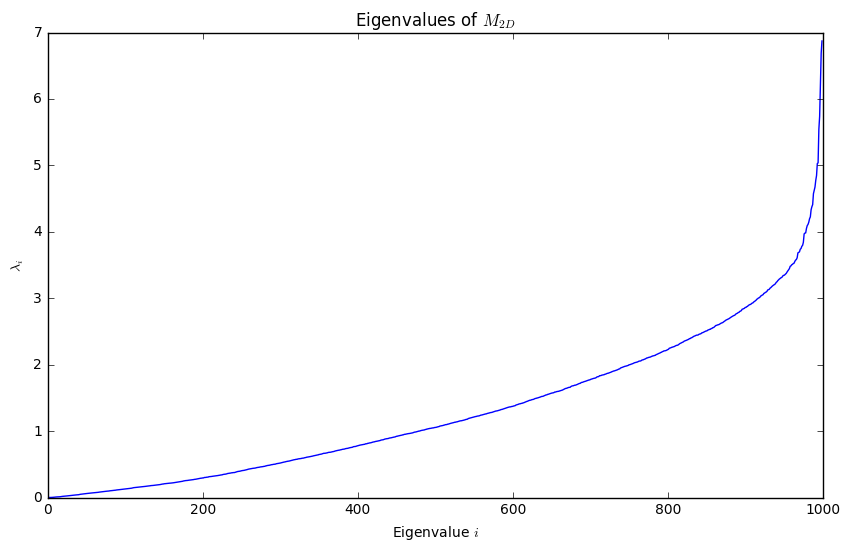
\includegraphics[width=1\linewidth]{images/matrix_eigenvalues}
    \caption{$M$ eigenvalues.}
    \label{fig:matrix_eigenvalues}
  \end{subfigure}
\caption{Matrix $M$ representations obtained for a 2D Locally Linear Embedding.}
\end{figure}

In Figure~\ref{fig:matrix_eigenvalues} there is plot the eigenvalues of the matrix $M$ which constantly increases until a point after the 900th eigenvalue that the values start increasing abruptly. The best option to choose the optimal embedding dimension will be to choose the \textit{i}th position where the knee is observed at the eigenvalues plot.

Other possible study to be made about the Locally Linear Embedding is see the effect of the number nearest neighbors used at the algorithm where the Nearest Neighbors are applied.

}
\problemAnswer{ % Answer

Regarding the embedding reconstruction, running the LLE algorithm with 8 nearest neighbors and embedding in 2D, I have tried the reconstruction of a sample inside the manifold, an another sample outside the manifold. On Figure~\ref{fig:reconstruction_inside_manifold} can be observed how a digit number $5$ has been reconstructed by the 8 nearest neighbors of the manifold. On the other hand, on Figure~\ref{fig:reconstruction_outside_manifold} can be observed how a point close the $0$ but placed outside the manifold is reconstructed but showing some malformation in the shape of the digit and also some discontinuities on the trace.

\begin{figure}[H]
  \begin{subfigure}{.25\textwidth}
    \centering
    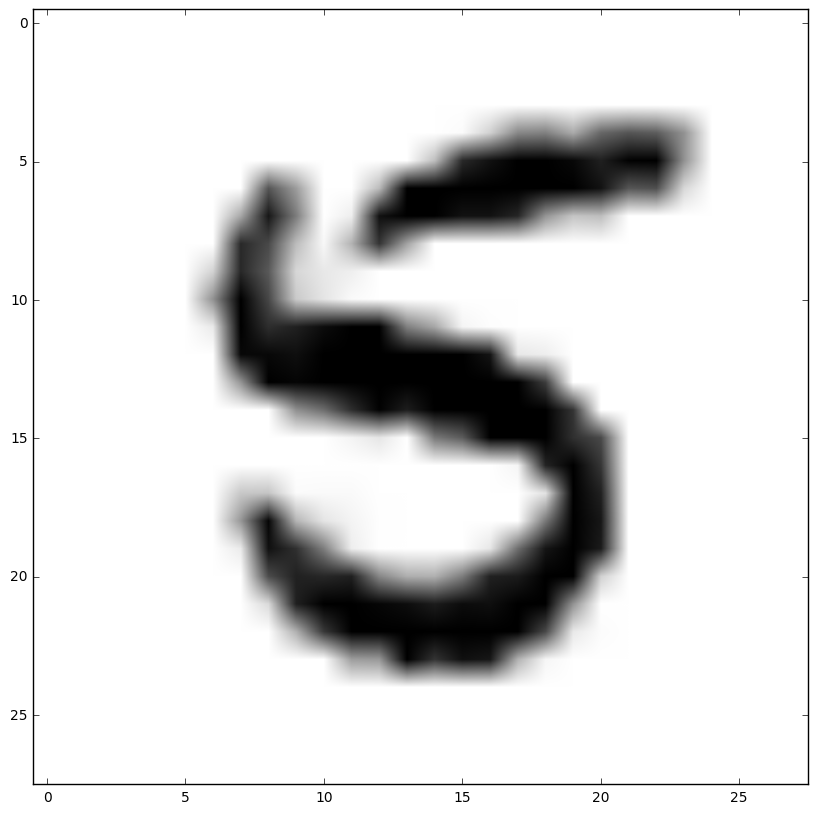
\includegraphics[width=1\linewidth]{images/reconstruction_inside_manifold}
    \caption{Reconstruction of a point inside the manifold.}
    \label{fig:reconstruction_inside_manifold}
  \end{subfigure}%
  \begin{subfigure}{.25\textwidth}
    \centering
    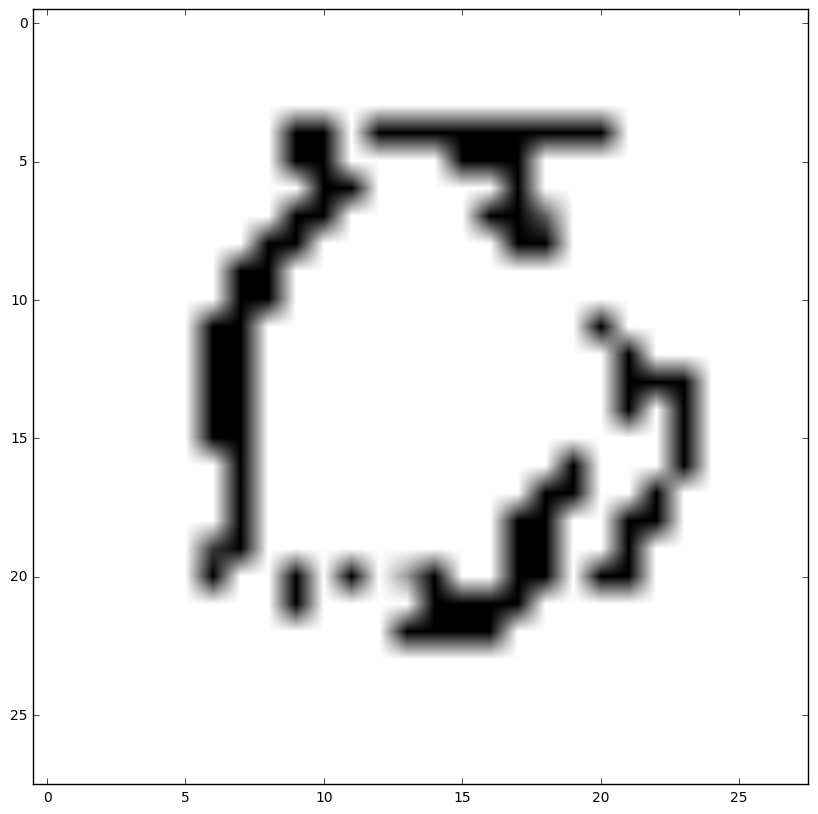
\includegraphics[width=1\linewidth]{images/reconstruction_outside_manifold}
    \caption{Reconstruction of a point outside the manifold.}
    \label{fig:reconstruction_outside_manifold}
  \end{subfigure}%
  \begin{subfigure}{.5\textwidth}
    \centering
    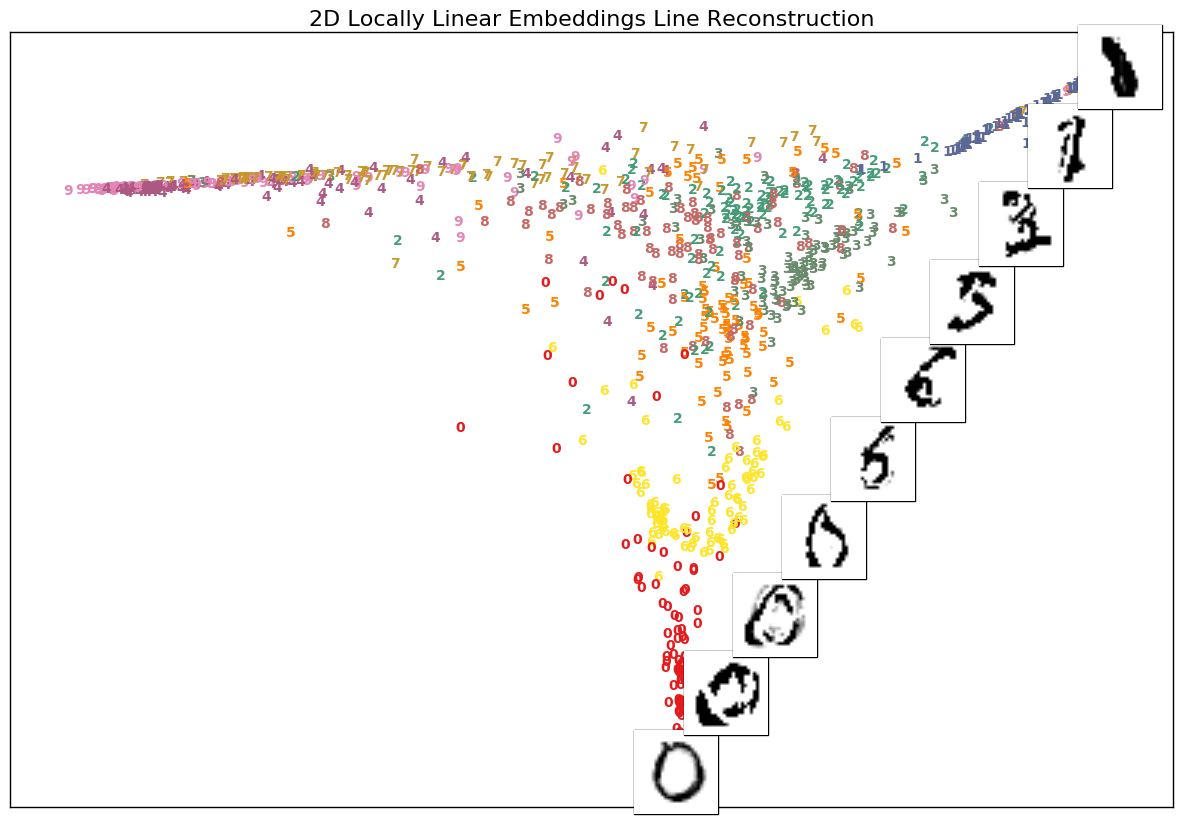
\includegraphics[width=1\linewidth]{images/reconstruction_line_manifold}
    \caption{Reconstruction of a line of points outside of the manifold.}
    \label{fig:reconstruction_line}
  \end{subfigure}
\caption{Reconstruction of points in the 2D embedding to the original space.}
\end{figure}

In addition, it has been drawn a line from two points crossing outside the manifold and reconstructing the middle points.
In Figure~\ref{fig:reconstruction_line} can be observed how the points reconstructed outside the manifold show the same characteristics as the one in Figure~\ref{fig:reconstruction_outside_manifold} but in addition it can be seen the evolution of the digit from 0 to 1 passing through 6, 5 and 3.

Finally, different distance measures have been tried to run the LLE algorithm. In Figure~\ref{fig:embeddings_metrics} can be found the 2D embedding for different metrics used: correlation between images, cosine distance and Manhattan or L1 distance respectively.

\begin{figure}[H]
  \begin{subfigure}{.33\textwidth}
    \centering
    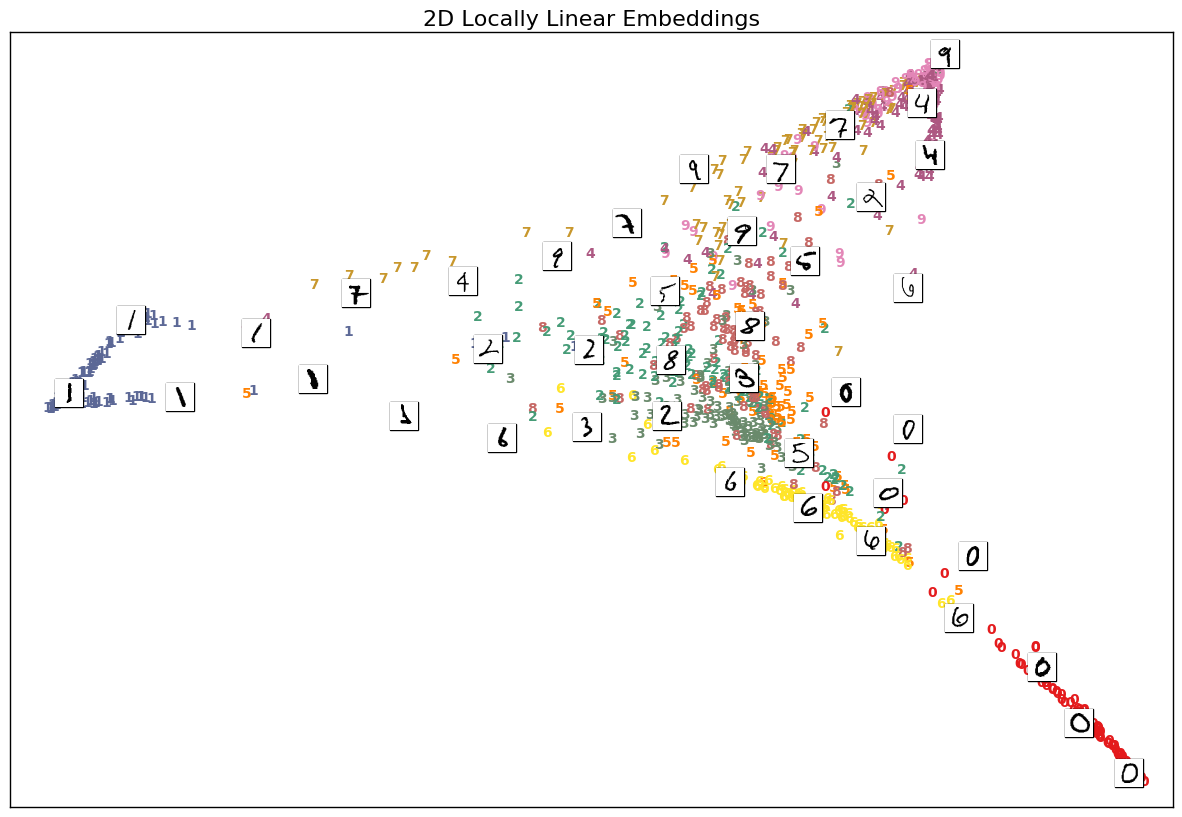
\includegraphics[width=1\linewidth]{images/2d_embeddings_correlation_metric}
    \caption{Correlation metric.}
  \end{subfigure}%
  \begin{subfigure}{.33\textwidth}
    \centering
    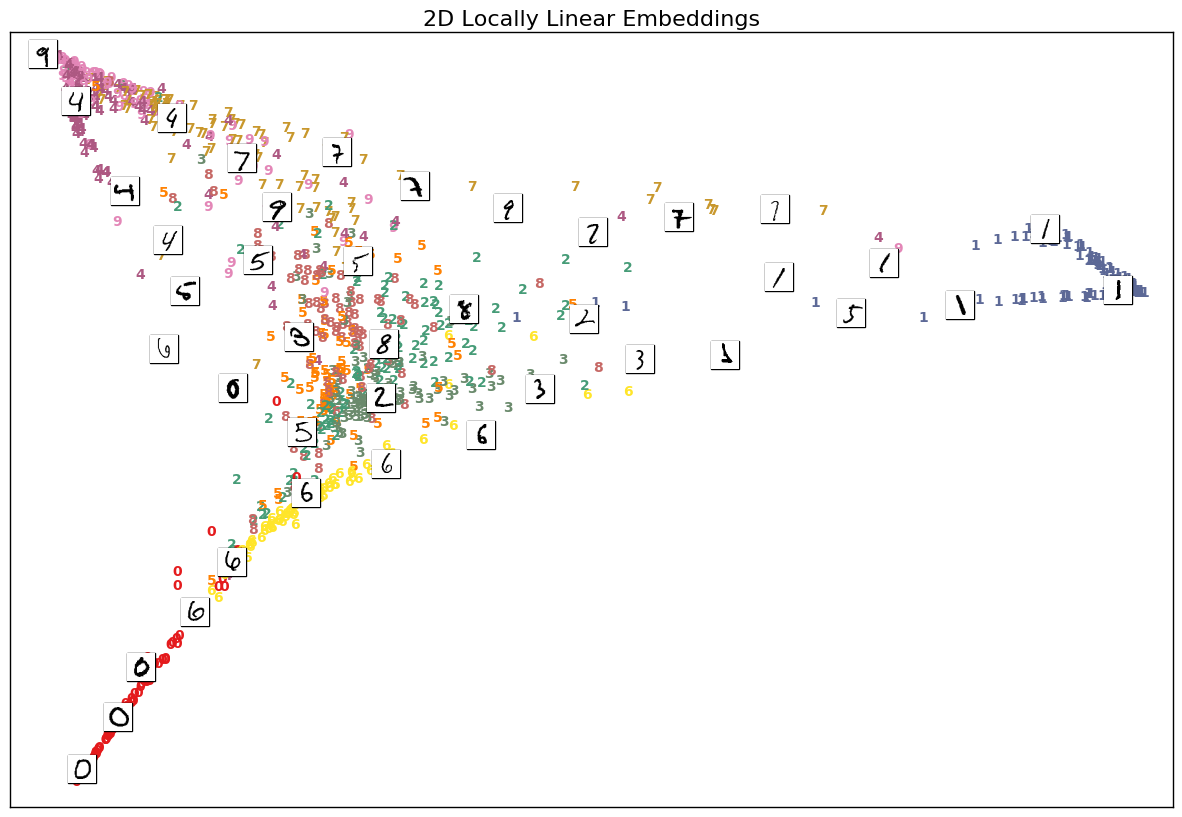
\includegraphics[width=1\linewidth]{images/2d_embeddings_cosine_metric}
    \caption{Cosine distance.}
  \end{subfigure}%
  \begin{subfigure}{.33\textwidth}
    \centering
    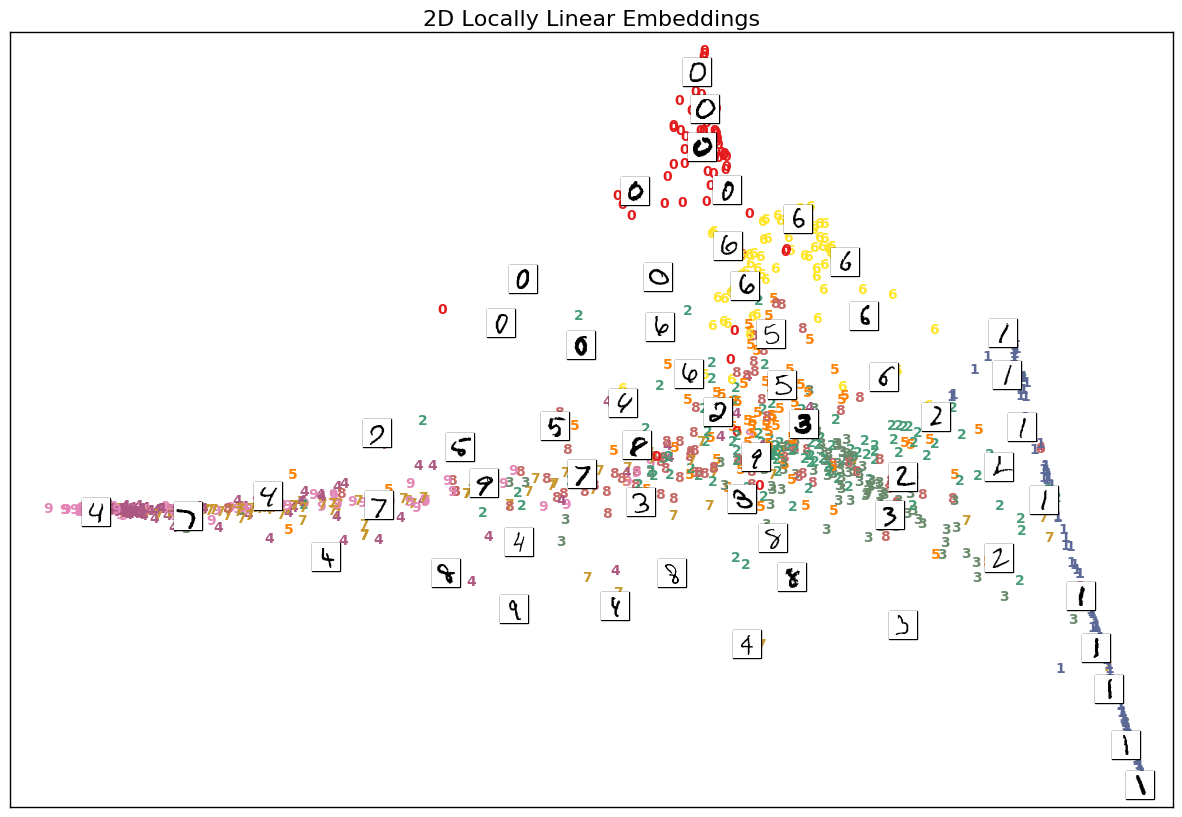
\includegraphics[width=1\linewidth]{images/2d_embeddings_l1_metric}
    \caption{L1 distance.}
  \end{subfigure}
  \caption{2D embedding for different metric/distance functions.}
  \label{fig:embeddings_metrics}
\end{figure}

For this three metrics, it can be observed how the clusters keep forming for each of the digits of the dataset, but change the shape of the embedded manifold.

}

\end{homeworkProblem}
\clearpage

%----------------------------------------------------------------------------------------
\begin{homeworkProblem}[The Implementation]
In the implementation section you give a concise insight to the practical aspects of this coding exercise. It mainly mentions the optimization methods used to solve the model equations. Did you encounter numerical or efficiency problems? If yes, how did you solve them?
Provide the link to your git branch of this coding exercise.\newline
Hard limit: One page

\vspace{10pt}
\problemAnswer{ % Answer

My current implementation is found on the git branch \hmwkGitBranch.

The implementation has not required further optimizations of the code. Working with 1000 samples it has been possible to work with dense arrays in a very precise and fast way even when $W$ matrix is very sparse.
For larger datasets, it would be necessary to work with sparse representation of this matrix in addition to use approximate methods to compute the eigenvalues and eigenvectors.
In addition to this, I have not encounter this problem but in case when the weights are computed, we found a $C$ singular matrix, it would be necessary to add a little regularization much lower than the trace as the original paper specify in the annex.
}
\end{homeworkProblem}
\clearpage

%----------------------------------------------------------------------------------------
\begin{homeworkProblem}[Your Page]
Your page gives you space to include ideas, observations and results which do not fall into the categories provided by us. You can also use it as an appendix to include things which did not have space in the other sections.\newline
No page limit.

\vspace{10pt}
\problemAnswer{ % Answer

I would like to add some results I get but I didn't found any reasonable explanation. Computing the reconstruction error agains the number of nearest neighbors used in the algorithm, I found that increasing the number of nearest neighbors, the reconstruction error tent to continuously decreasing such as shown in Figure~\ref{fig:reconstruction_error_knn}.
This does not make any sense because I found some equivalent computations in the literature\footnote{http://jultika.oulu.fi/files/isbn9514280415.pdf} where they find a minimum corresponding an optimal $K$ for the nearest neighbor where the reconstruction error of the embedding was minimum. Also I haven't found the sense to thus results because if I execute the code with 50 nearest neighbors for examples, the resulting 2D embedding consist in a uniform cloud where no clusters can be found such as in Figure~\ref{fig:embedding_50_nn}.

\begin{figure}[H]
    \centering
    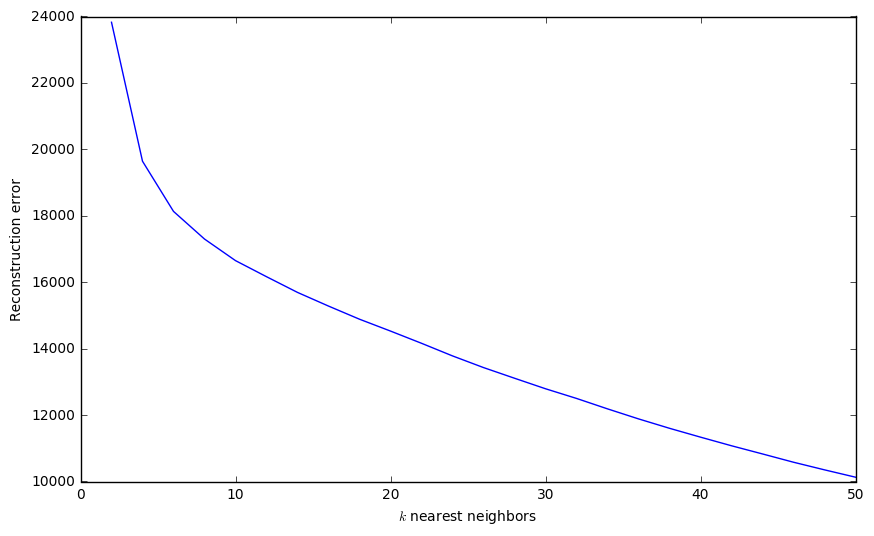
\includegraphics[width=0.7\linewidth]{images/reconstruction_error_knn}
    \caption{Reconstruction error against the number of Nearest Neighbors.}
    \label{fig:reconstruction_error_knn}
\end{figure}

\begin{figure}[H]
    \centering
    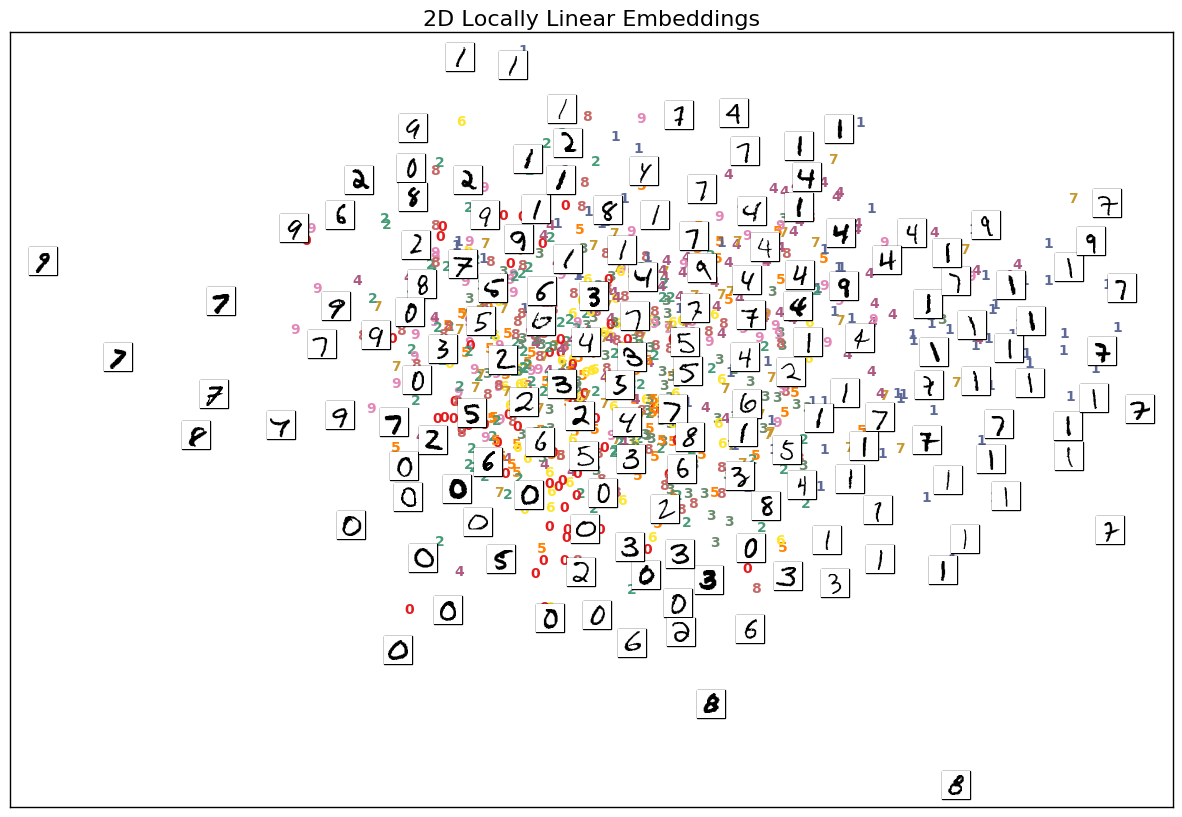
\includegraphics[width=0.7\linewidth]{images/2d_embeddings_50_nn}
    \caption{2D Embedding space using 50 nearest neighbors.}
    \label{fig:embedding_50_nn}
\end{figure}

}
\end{homeworkProblem}
\clearpage

\end{document}
